% !TeX encoding = UTF-8
% @Yongjian.Li 澳門科技大學-畢業論文 LaTeX template-2023

% User's Guide: 
    % https://iihciyekub.github.io/must-thesis-manual
% Github: 
    % https://github.com/iihciyekub/MUST-Thesis
% Overleaf: 
    % https://www.overleaf.com/read/mjzpcxztzqzv
% Overleaf project 使用的 chrome 浏览器扩展程序 overleaf s2t/bib2bbl, 下载地址:
    % https://chrome.google.com/webstore/detail/overleaf-s2tbib2bbl/icekiliecbhnockmfkehoebbkmhmapmo?hl=zh-CN
% bib2bbl online: 
    % https://pychat.online/bib2bbl

% 最後更新: 2023-5-08

\documentclass[
    writingLanguage=english, 
    addPageTitle=on,
    addDeclaration=on,
    addMUSTlog=off,
    printing=off,
    refIndent=on,
    addFigTOC=on,
    addTabTOC=on,
]{.def/must}


% 論文基本信息,必填不能刪除
\def\shool              {Macau University of Science and Technology}
\def\cnTitle            {XXX 銀行(澳門分行)與 XXX 銀行合併之研究}
\def\cnShortTitle       {\cnTitle}% 页眉显示的中文论文短题目
\def\enTitle            {The Study on the Relationship between Social Responsibility and Organizational Trust}
\def\enShortTitle       {The Study on the Relationship between SR \& OT}% 页眉显示的英文论文短题目
\def\Name               {Name}% 名稱
\def\StudentNo          {Student No.}% 學號
\def\Faculty 	        {Faculty of Business Administration}% 所在學院
\def\Program 	        {Program}% 學位名稱
\def\Major              {Major}% 專業名稱
\def\Supervisor	        {Supervisor}% 指導老師
\def\DateofWriting		{\datea\today}% 設置論文寫作完成時間
\def\DateofDeclaration	{\dateb\today}% 設置論文原創聲明時間
\def\DateofSignature	{2023/06/30}% 設置簽署論文原創聲明的時間
\def\PublicAfterYears   {5}% 設置論文幾年後公開




 
\begin{document}


\begin{abstract@en}{keyword1,keyword1,keyword1,keyword1,}
\txtHere{1-3}

\the\baselineskip
\end{abstract@en}

% 添加目錄 
\addtableofcontents


\chapter{Introduction}
\txtHere{1}
\section{Research Aim and Objectives}
\section{fig}
\captionsetup[figure]{singlelinecheck=off,justification=raggedright}
\captionsetup[subfigure]{singlelinecheck=on}
\tikzstyle{every pin}=[fill=white,draw=black,font=\small,]
\begin{figure}[H]
	\centering
	\begin{subfigure}{0.49\textwidth}
	  	\centering
		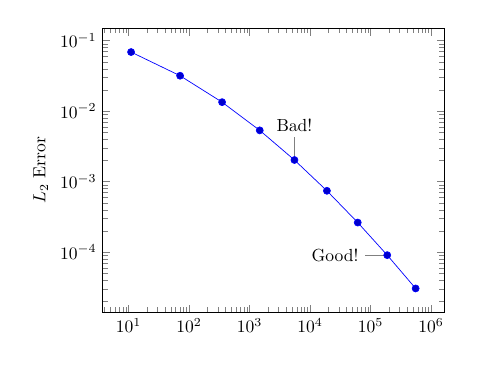
\begin{tikzpicture}[scale = 0.63276]
			\begin{loglogaxis}[
				%xlabel={\textsc{Dof}},
				ylabel={$L_2$ Error},
				]
				\addplot coordinates {
					(11, 6.887e-02)
					(71, 3.177e-02)
					(351, 1.341e-02)
					(1471, 5.334e-03)
					(5503, 2.027e-03)
					(18943, 7.415e-04)
					(61183, 2.628e-04)
					(187903, 9.063e-05)
					(553983, 3.053e-05)
				};
				\node [coordinate,pin=above:{Bad!}]
				at (axis cs:5503,2.027e-03) {};
				\node [coordinate,pin=left:{Good!}]
				at (axis cs:187903,9.063e-05) {};
			\end{loglogaxis}
		\end{tikzpicture}
		\caption{A subfigure}
		\label{fig:sub1}
	\end{subfigure}
	\hfill
	\begin{subfigure}{.49\textwidth}
		\centering
		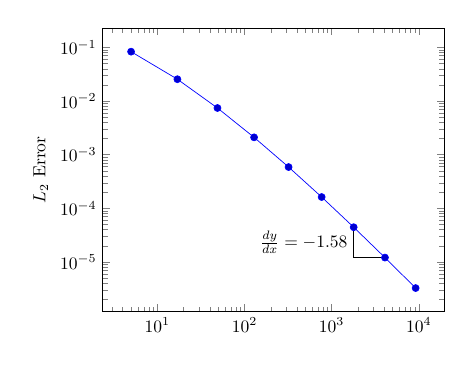
\begin{tikzpicture}[scale = 0.63276]
			\begin{loglogaxis}[
				ylabel=$L_2$ Error,
				]
				\draw
				(1793,4.442e-05)
				|- (4097,1.207e-05)
				node [near start,left]
				{$\frac{dy}{dx} = -1.58$};
				\addplot coordinates {
					(5, 8.312e-02)
					(17, 2.547e-02)
					(49, 7.407e-03)
					(129, 2.102e-03)
					(321, 5.874e-04)
					(769, 1.623e-04)
					(1793, 4.442e-05)
					(4097, 1.207e-05)
					(9217, 3.261e-06)
				};
			\end{loglogaxis}
		\end{tikzpicture}
		\caption{A subfigure}
	  	\label{fig:sub2}
	\end{subfigure}\\

	\begin{subfigure}{.49\textwidth}
		\centering
		\includegraphics[width=.5\linewidth]{.def/.resource/eg05.png}
		\caption{A subfigure}
		\label{fig:sub3}
	\end{subfigure}
	\begin{subfigure}{.49\textwidth}
		\centering
		\includegraphics[width=.5\linewidth]{.def/.resource/eg06.png}
		\caption{A subfigure}
		\label{fig:sub4}
	\end{subfigure}
	\caption{A figure with two subfigures}
	\label{fig:sub}
\end{figure}
 
subfig\ref{fig:sub1}subfig\ref{fig:sub2}subfig\ref{fig:sub3}subfig\ref{fig:sub4}



\section{table}

\captionsetup[table]{singlelinecheck=off,justification=raggedright}
\begin{table}
\caption{this is table data}
\centering
\begin{tabularx}{\textwidth}{XXX} % 表格寬度為網頁的一半
\toprule
content & content & content \\
\midrule
row1 & row1 & row1\footnote{footnote} \\
row2 & row2 & row2 \\
\bottomrule
\end{tabularx}
\caption*{this is footnote}
\end{table}




\subsection{Background}
\txtHere{1}\citep{cohen2007, harvey2007, manguel2009, šteger2010, Villazón2011, bordwell2013, cole2013, deliot2014, foster2017, paige2017, johnson2018, wipawin2018, poff2019, giles2019, TaiwanNews2019, abdoh2019, macdonald2020, Milliot2020, OrganisationforEconomicCo2020, rothfeld2020, crotty2020, melero2021}

\subsection{Current State}
\txtHere{1}

\chapter{Related Work}
\txtHere{1}
\section{Previous Studies}
\txtHere{1}
\subsection{Study 1}
\txtHere{1}
\subsection{Study 2}
\txtHere{1}
\subsection{Study 3}
\txtHere{1}
\section{Limitations of Previous Studies}
\txtHere{1}

\begin{equation}
V_0=X_0(1-T)(1-b) \sum_{t=1}^n \frac{(1+g)^t}{(1+k)^t}+\frac{X_0(1-T)(1-g)^{n+1}}{k(1+k)^n}
\end{equation}


\begin{axiom}
Theorem 4.1. Let $F(\Lambda)=(R-v-r-c) \Lambda-2 \sqrt{h c \Lambda}$. The social welfare solution is to set $\mu_1=\mu_2=\lambda_1=\lambda_2=0$ if $F(\Lambda)<\sigma$; otherwise, to set $\lambda_i=\Lambda, \mu_i=\Lambda+\sqrt{h \Lambda / c}$, $\mu_j=\lambda_j=0$, for either $i=1$ or 2 with corresponding $j \neq i$.
\end{axiom}


\begin{theorem}
For the capacity choice problem, four
cases may arise.
\begin{enumerate}[itemsep=2pt,topsep=0pt,parsep=0pt,leftmargin=*,label=\emph{(\roman*)}]
    \item If $F(\Lambda)<\sigma$, then the unique equilibrium is such that none of the firms would operate in the market, i.e., $p_1=p_2=0$ and $\mu_1=\mu_2=0$, and the corresponding $\lambda_1=\lambda_2=0$.
    \item If $F(\Lambda / 2)<\sigma \leqslant F(\Lambda)$, then there are two equilibria, each corresponding to one of the firms to operate in the market. The firm enters the market captures the whole market and sets monopoly capacity and price, i.e.,
\end{enumerate}

\end{theorem}


\begin{definition}
 definition。
\end{definition}


\begin{example}
 example。
\end{example}



\begin{property}
 property。
\end{property}

\begin{proposition}
 proposition。
\end{proposition}


\begin{lemma}
 lemma。
\end{lemma}

\begin{corollary}
 corollary。
\end{corollary}

\begin{remark}
 remark。
\end{remark}



\begin{condition}
 condition。
\end{condition}



\begin{conclusion}
 conclusion。
\end{conclusion}


\begin{assumption}
 assumption。
\end{assumption}






\section{funation}









\chapter{math fun}
\begin{equation}
\label{eq1}
e^{\pi i}+1=0
\end{equation}
\begin{align}
2 y & =d\label{eq:IntoSection}\\
3 y & =cx+d\\
4 y_{12} & =bx^{2}+cx+d\\
5 y(x) & =ax^{3}+bx^{2}+cx+d
6 
\end{align}
\begin{equation}
2 x=\left\{ \begin{array}{cl}
3 0 & \textrm{if }A=\ldots\\
4 1 & \textrm{if }B=\ldots\\
5 x & \textrm{this run  text.}\end
{array}\right.
\end{equation}       


\subsection{alg}

 





\chapter{Methodology}
\txtHere{1}
\section{Research Design}
\txtHere{1}
\subsection{Experimental Design}
\txtHere{1}
\subsection{Sampling Method}
\txtHere{1}
\section{Data Collection}
\txtHere{1}
\subsection{Data Sources}
\txtHere{1}
\subsection{Data Collection Procedures}
\txtHere{1}
\section{Data Analysis}
\txtHere{1}
\subsection{Statistical Analysis}
\txtHere{1}
\subsection{Qualitative Analysis}

\chapter{Results}
\txtHere{1}
\section{Descriptive Statistics}
\txtHere{1}
\subsection{Frequencies}
\txtHere{1}
\subsection{Measures of Central Tendency}
\txtHere{1}
\subsection{Measures of Dispersion}
\txtHere{1}
\section{Inferential Statistics}
\txtHere{1}
\subsection{Hypothesis Testing}
\txtHere{1}
\subsection{Regression Analysis}
\txtHere{1}
\subsection{Factor Analysis}
\txtHere{1}

\chapter{Discussion}
\txtHere{1}
\section{Interpretation of Results}
\txtHere{1}
\subsection{Implications of Results}
\txtHere{1}
\subsection{Limitations of Study}
\txtHere{1}
\section{Contributions to the Field}
\txtHere{1}
\subsection{Recommendations for Future Research}
\txtHere{1}
\chapter{Conclusion}
\txtHere{1}
\section{Summary of Findings}
\txtHere{1}
\section{Conclusions}
\txtHere{1}
\section{Limitations of Study}
 \txtHere{1}
\txtHere{1}
\section{Implications for Practice}
\txtHere{1}




% 請確保bib 文件名稱為 ref.bib, 利用js文件處理後的bbl文件名稱為 ref.bbl
\addreference

\begin{appendix}

\end{appendix}


\begin{acknowpage}

\end{acknowpage}











% ---- >>start
\begin{addcvpage}
% 設置入學時間
\addedudate{Sept, 2019}

% 填寫教育經歷,注意內容以逗號作分隔,
\addeduItem{2009.16-2012.13,Macau University of Science and Technology, Faculty of Business, Taipa Island, Macau, China.}
\addeduItem{2009.16-2012.13,Macau University of Science and Technology, Faculty of Business, Taipa Island, Macau, China.}
\addeduItem{2009.16-2012.13,Macau University of Science and Technology, Faculty of Business, Taipa Island, Macau, China.}

%增加學術文章
\addpaperItem{ 
    \item  Macau University of Science and Technology, Taipa Island, Macau, China.,
    \item Macau University of Science and Technology, Taipa Island, Macau, China.,
}

% 增加項目
\addprojectItem{
    \item 中國澳門氹仔島澳門科技大學,商學院商學院
    \item 商學院商學院商學院中國澳門氹仔島澳門科技大學,商學院商學院商學院商學院商學院中國澳門氹仔島澳門科技大學,商學院商學院商學院商學院商學院
}
\end{addcvpage}
% << ----end







\end{document}